\section{Another important celestial parameter: the obliquity}
\label{obliquity}

This section describes the implementation of the obliquity and the explanation of the impact on the surface temperature. The obliquity is defined as the angle of tilt of the body's axis of rotation. Thus, it has an immediat impact on the repartition of temperature on the body as this figure describes: 
\begin{center}
    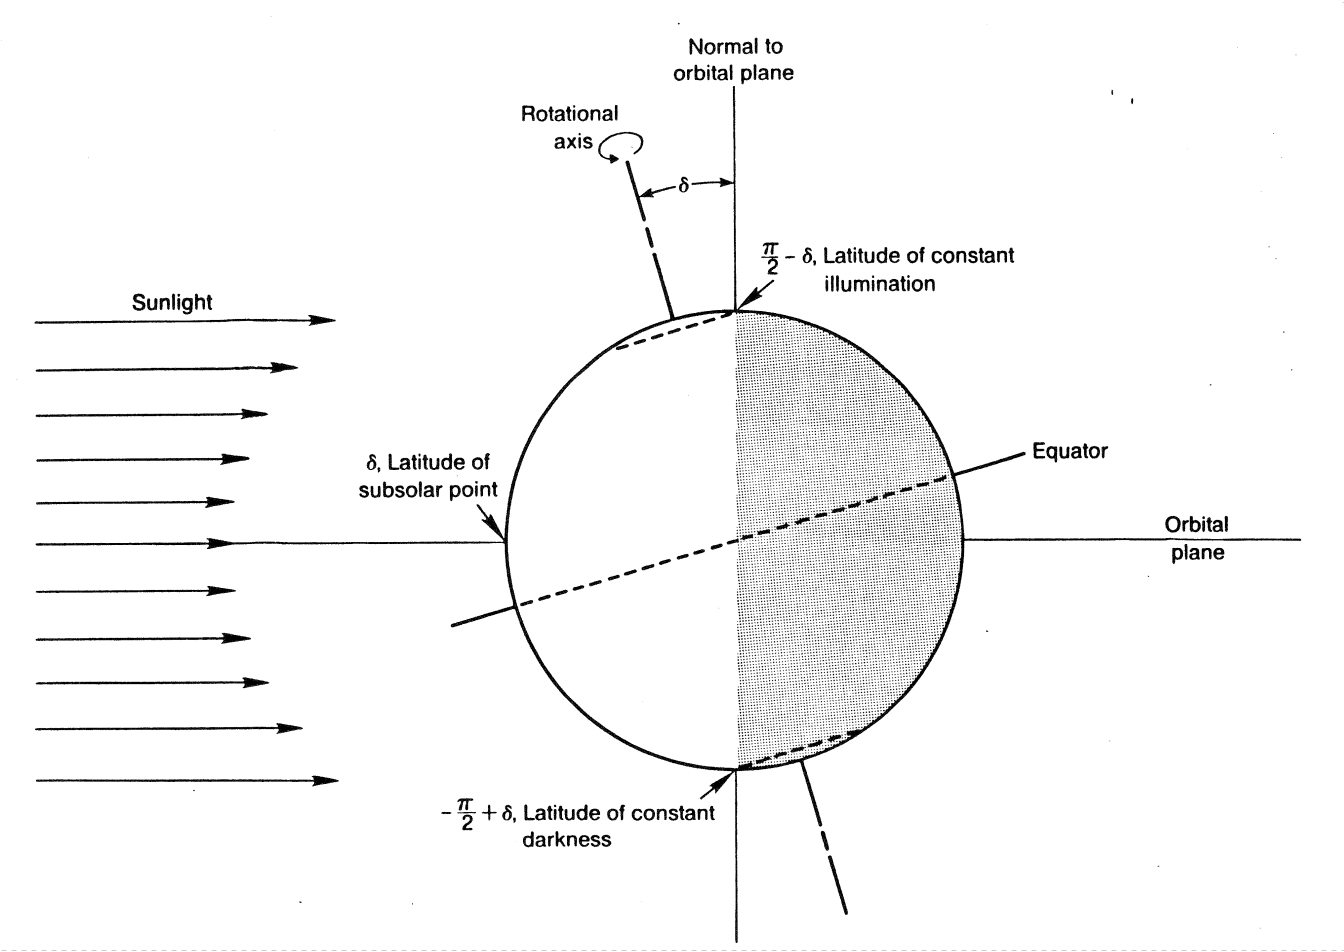
\includegraphics[width=\linewidth]{rsc/obliquity.png}
    \captionof{figure}{Representation of the obliquity with the orbital plane and the rotational axis}
\end{center}
The subsolar point is not anymore located on the equator. Depending on the position of the asteroid on its orbit, only one pole is not receiving direct heating from the Sun.
\begin{center}
    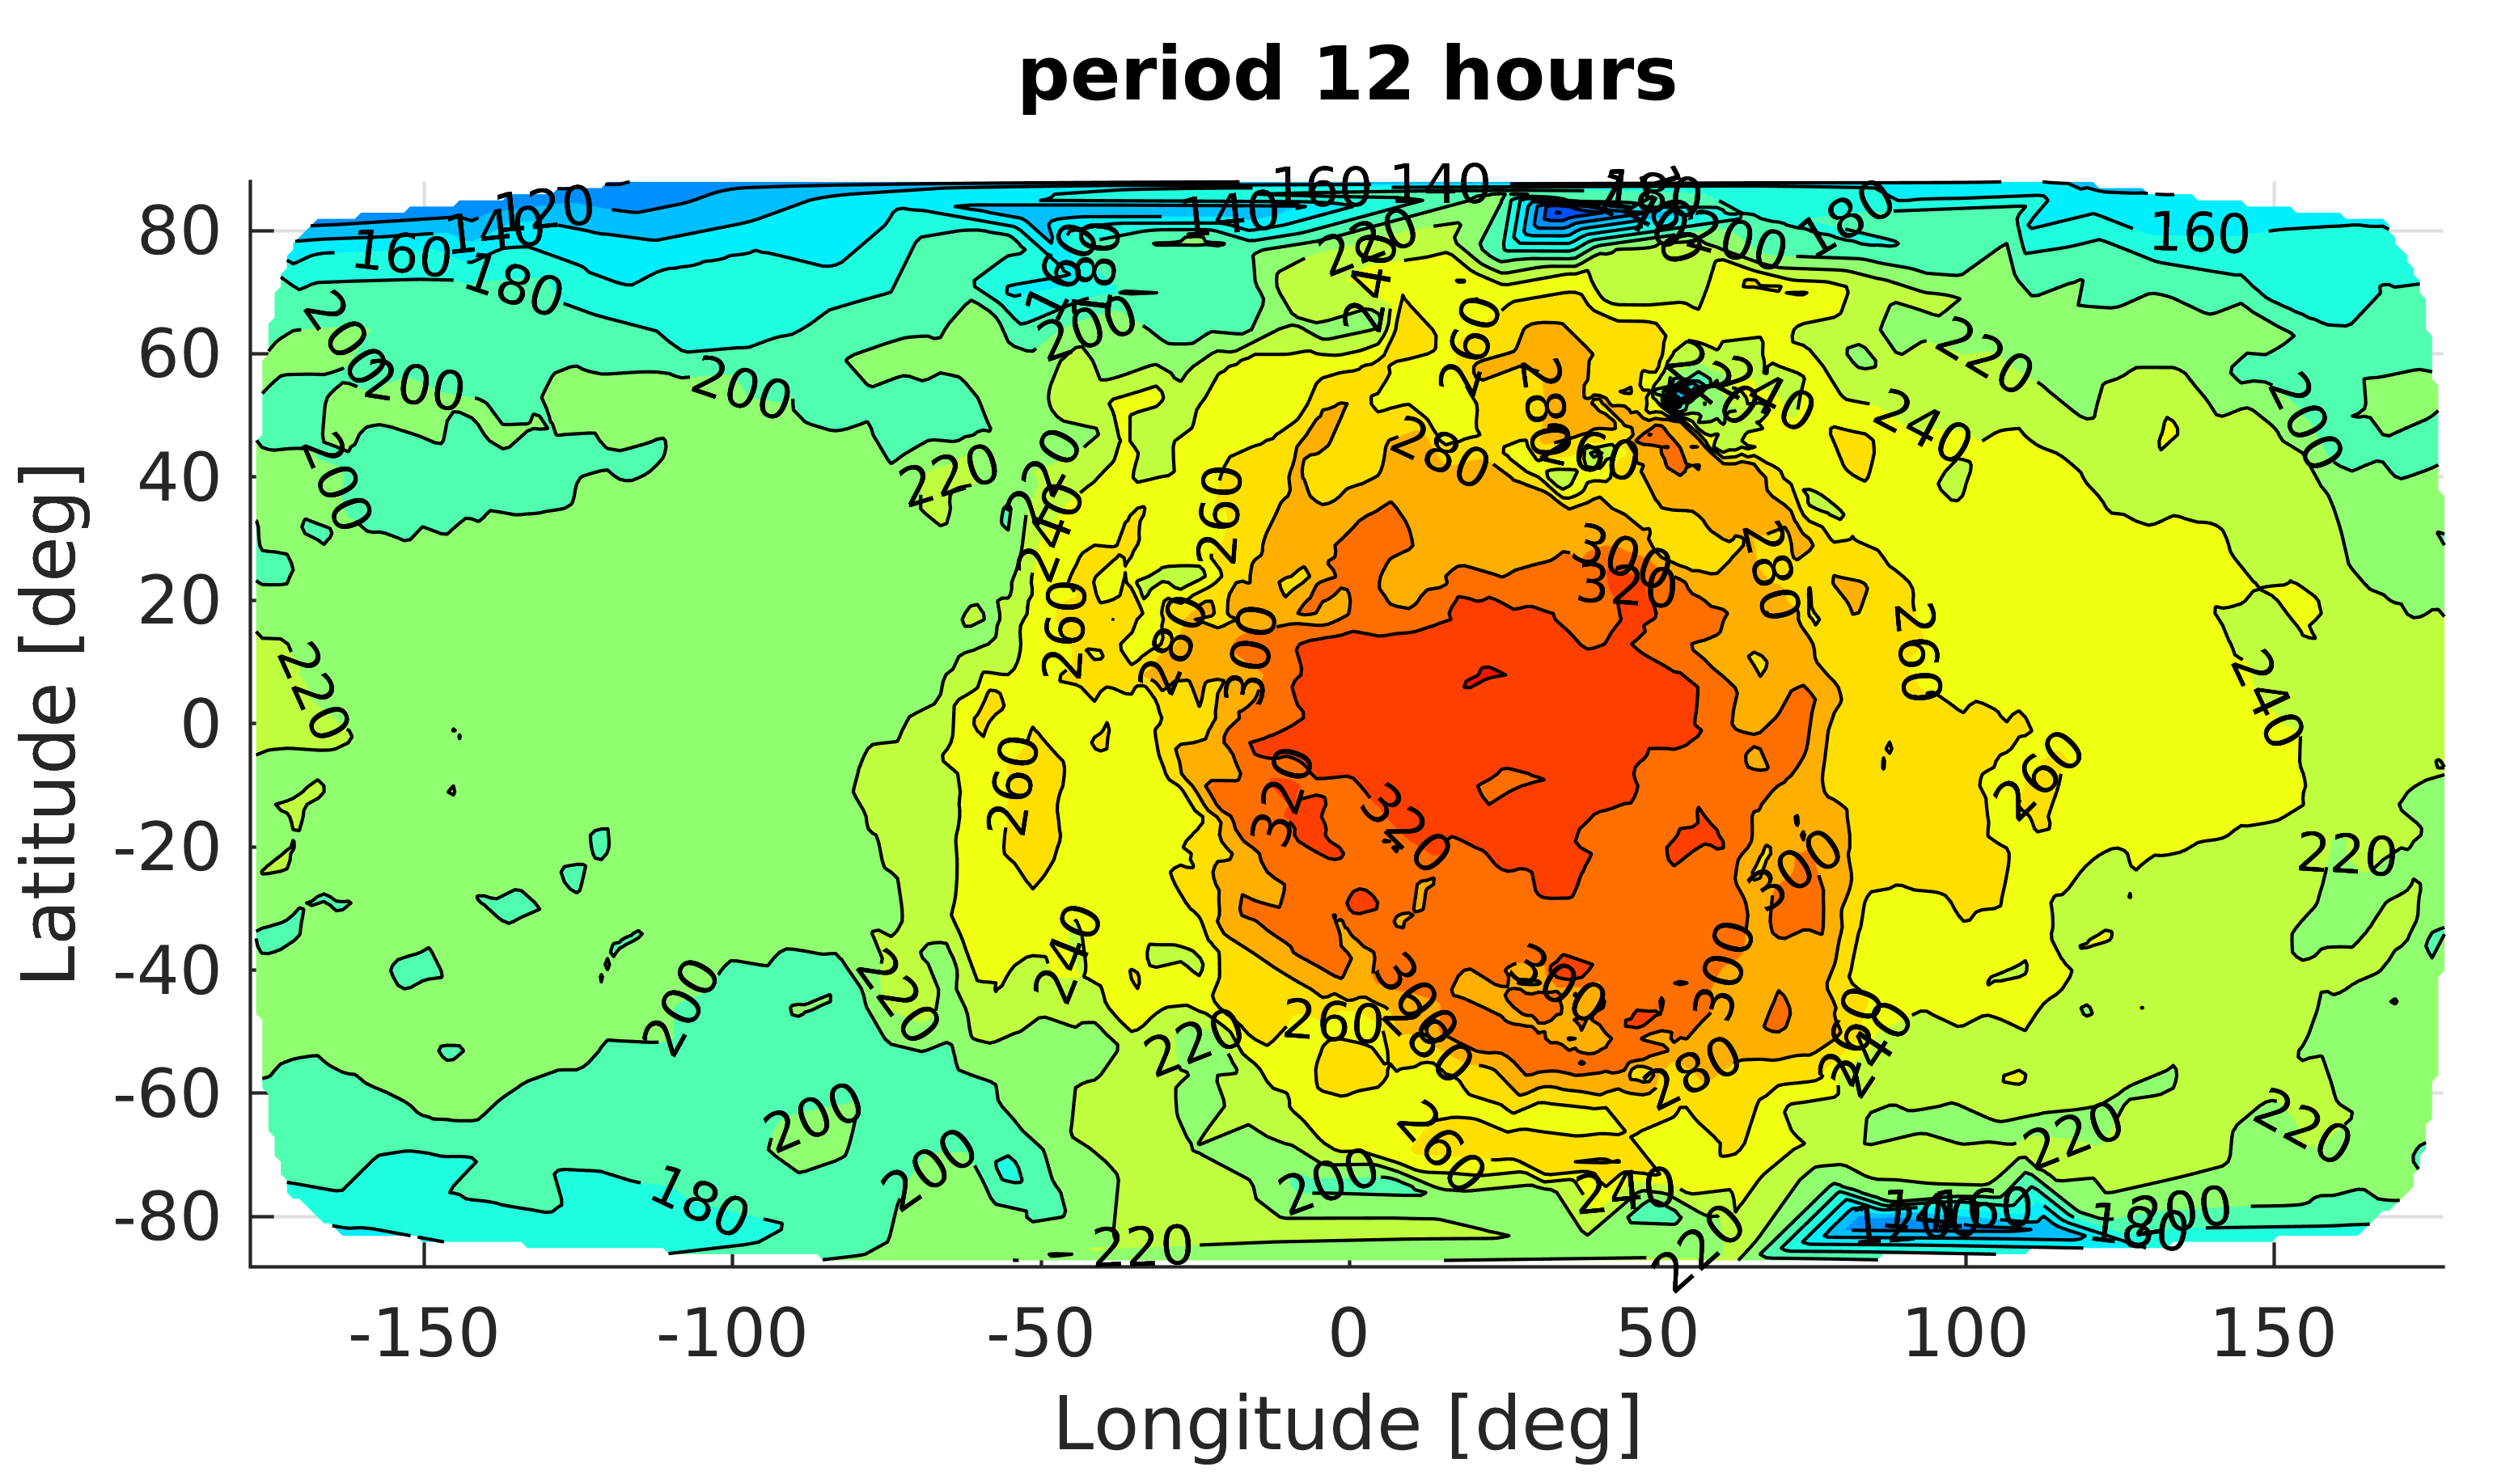
\includegraphics[width=\linewidth]{rsc/theo12h.png}
    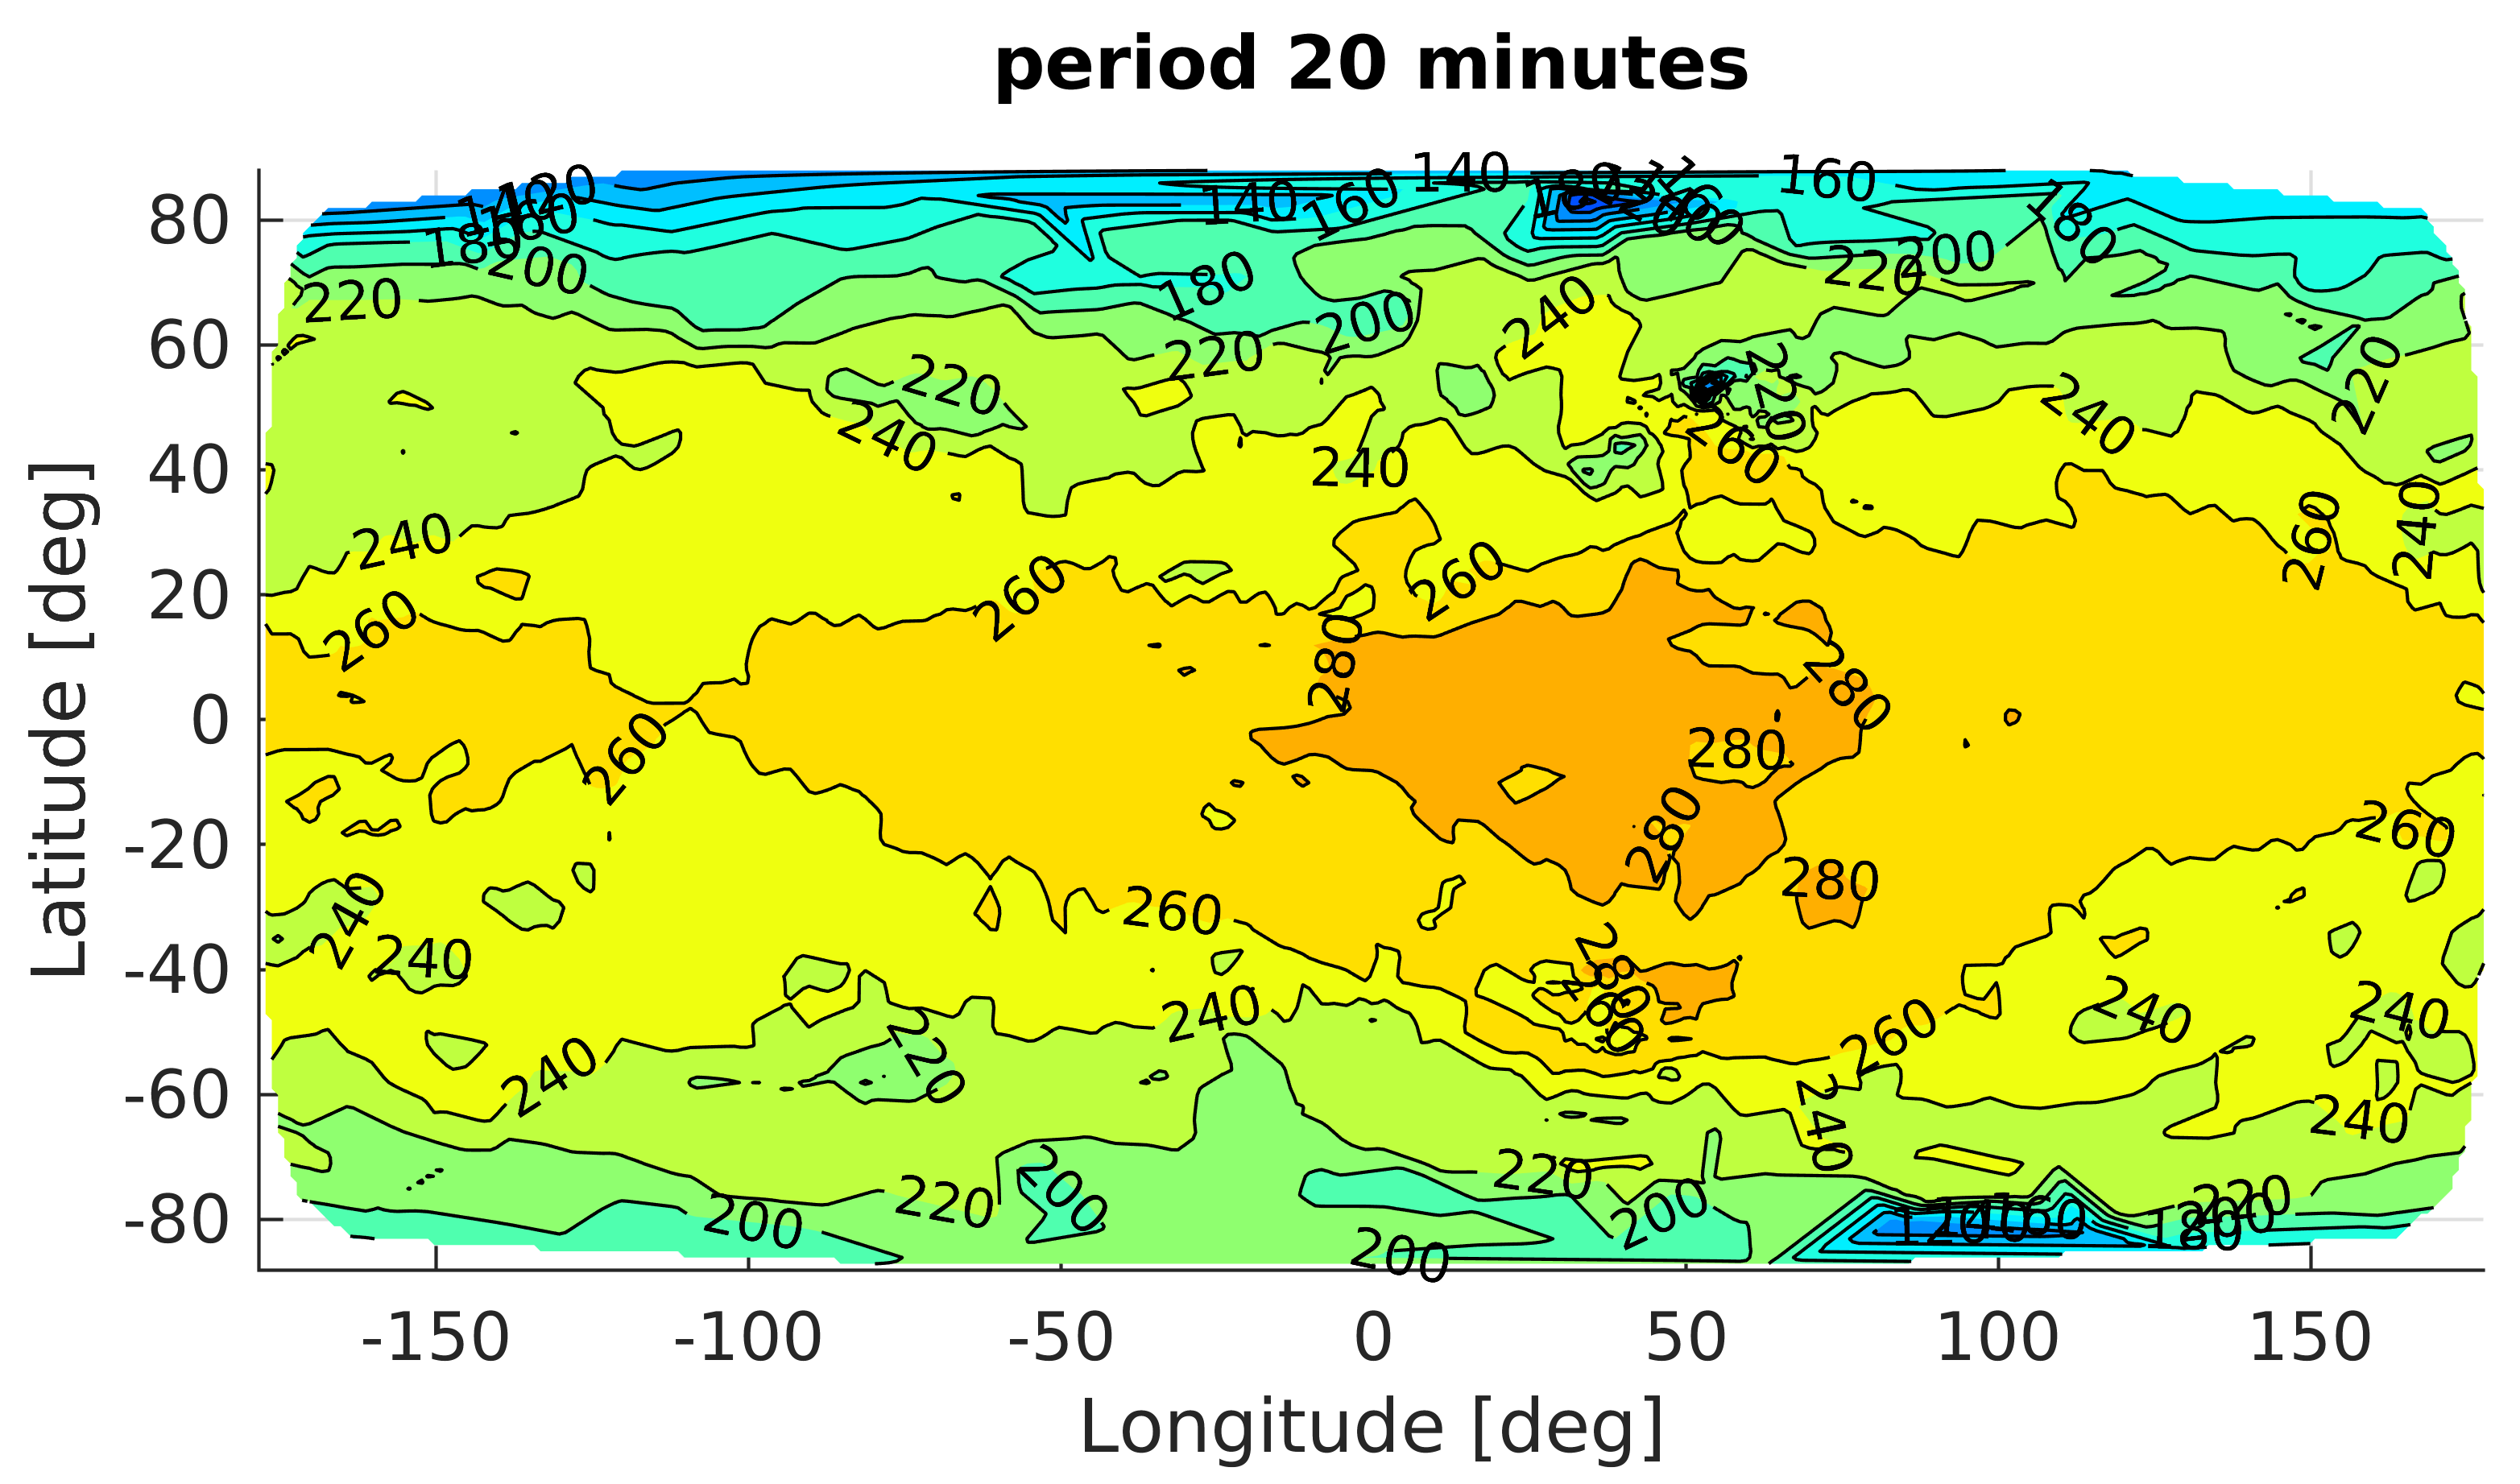
\includegraphics[width=\linewidth]{rsc/theo20mn.png}
    \captionof{figure}{HO3}
\end{center}
